\section{Ratio of Cross-Section Determination}
\label{RCS}
\def\effTot{\ensuremath{\epsilon_{\mathrm{tot}}}\xspace}
\def\effTotJ{\ensuremath{\epsilon_{\mathrm{tot,\jpsi}}}\xspace}
\def\effTotP{\ensuremath{\epsilon_{\mathrm{tot,\psitwos}}}\xspace}
\def\effAcc{\ensuremath{\epsilon_{\mathrm{acc}}}\xspace}
\def\effReco{\ensuremath{\epsilon_{\mathrm{Reco\&Sel}}}\xspace}
\def\effID{\ensuremath{\epsilon_{\mathrm{MuonID}}}\xspace}
\def\effTrigger{\ensuremath{\epsilon_{\mathrm{Trigger}}}\xspace}
The double differential cross-section for prompt and non-prompt $\jpsi$ and \psitwos production in a given multiplicity bin is defined as
\begin{equation}
    \frac{\deriv^2\sigma}{\deriv y\deriv \pt}
    = \frac{N}
           {\mathcal{L}\times\effTot\times \BR \times\Delta y \times \Delta \pt}.
  \label{CrossSecJ}
\end{equation}
where $N$ is the number of candidates obtained by fit, $\mathcal{L}$ is the integrated luminosity, \effTot is the total efficiency in the multiplicity bin, $\Delta\pt$ is the bin width of the transverse momentum and $\Delta y$ is the bin width of the rapidity. $\BR(\jpsi\rightarrow\mu^+\mu^-)=(5.961\pm0.033)\%$ is the branching fraction of the decay $\jpsi\rightarrow \mu^+ \mu^-$, and the assumption of lepton universality allows to use  $\BR(\psitwos\rightarrow e^+e^-)=(7.93\pm0.17)\times10^{-3}$ instead of the branching fraction of \psitwos to dimuon decay, taking advantage of the small uncertainties. 

The double differential ratio in a given multiplicity bin is further defined by,
\begin{equation}
    \frac{\sigma_{\psitwos}}{\sigma_{\jpsi}} =
    \frac{N_{\psitwos}}{N_{\jpsi}} \times
    \frac{\effTotJ} {\effTotP} \times
    \frac{\mathcal{B}_{\jpsi \rightarrow \mu^+ \mu^-}}{\mathcal{B}_{\psitwos\rightarrow e^+e^-}}.
    \label{Rsingle}
\end{equation}
The yield of prompt and from-$b$ charmonia is determined through a two-dimensional extended unbinned maximum likelihood fit. This fit is conducted on the distributions of the invariant mass $m_{\mu^+\mu^-}$ and pseudo decay time $t_z$ of the candidates. For the mass spectrum of signals, double Crystal Ball function is employed for \jpsi, sharing a common mean but having distinct widths, and single Crystal Ball function for \psitwos, the relation between width and tail positions is determined through simulations. The background mass spectrum is described using an exponential decay with an adjustable slope parameter. As for the $t_z$ distributions, prompt and from-$b$ charmonia are characterized by a Dirac $\delta$ function and an exponential function, respectively, both convolved with a shared double-Gaussian resolution function. The background $t_z$ distribution is parameterized using an empirical function, consisting with three positive and two negative exponential functions, each convolved with a double Gaussian function. The parameters for the background shape are determined from fits to data in mass sideband regions $|m_{\mu^+\mu^-}-m_{\jpsi}^{PDG}|>60\mevc$ and $|m_{\mu^+\mu^-}-m_{\psitwos}^{PDG}|>60\mevc$, where mostly background candidates are present. The shape parameters for $t_z$ background are fixed in the final two-dimensional fit. An example of a two-dimensional fit projected onto mass and $t_z$ spectra is presented in Figure~\ref{fig:2Dtz}.
\begin{figure}[!tbp]
  \begin{center}
    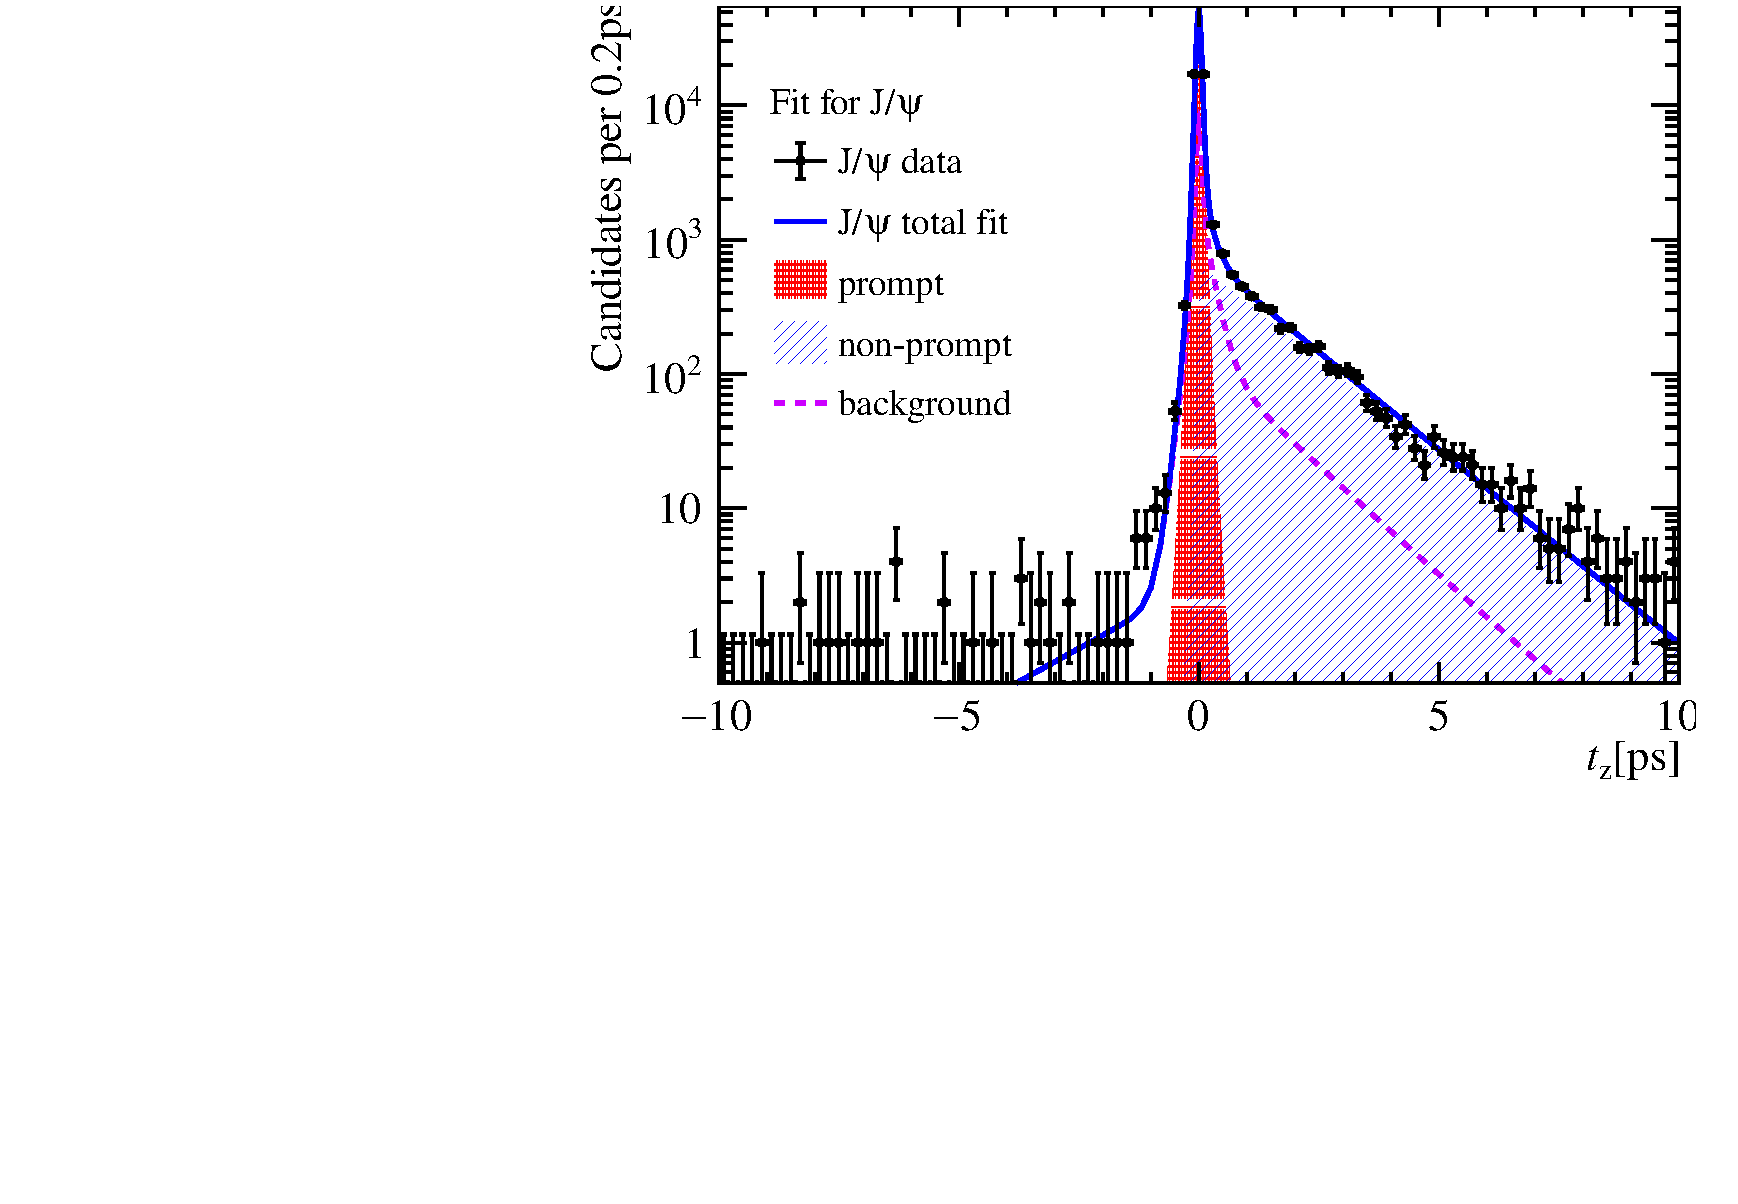
\includegraphics[width=0.49\linewidth]{pdf/pPb/Workdir/TwoDimFit/ProjTz/Jpsi_n2y1pt1.pdf}
    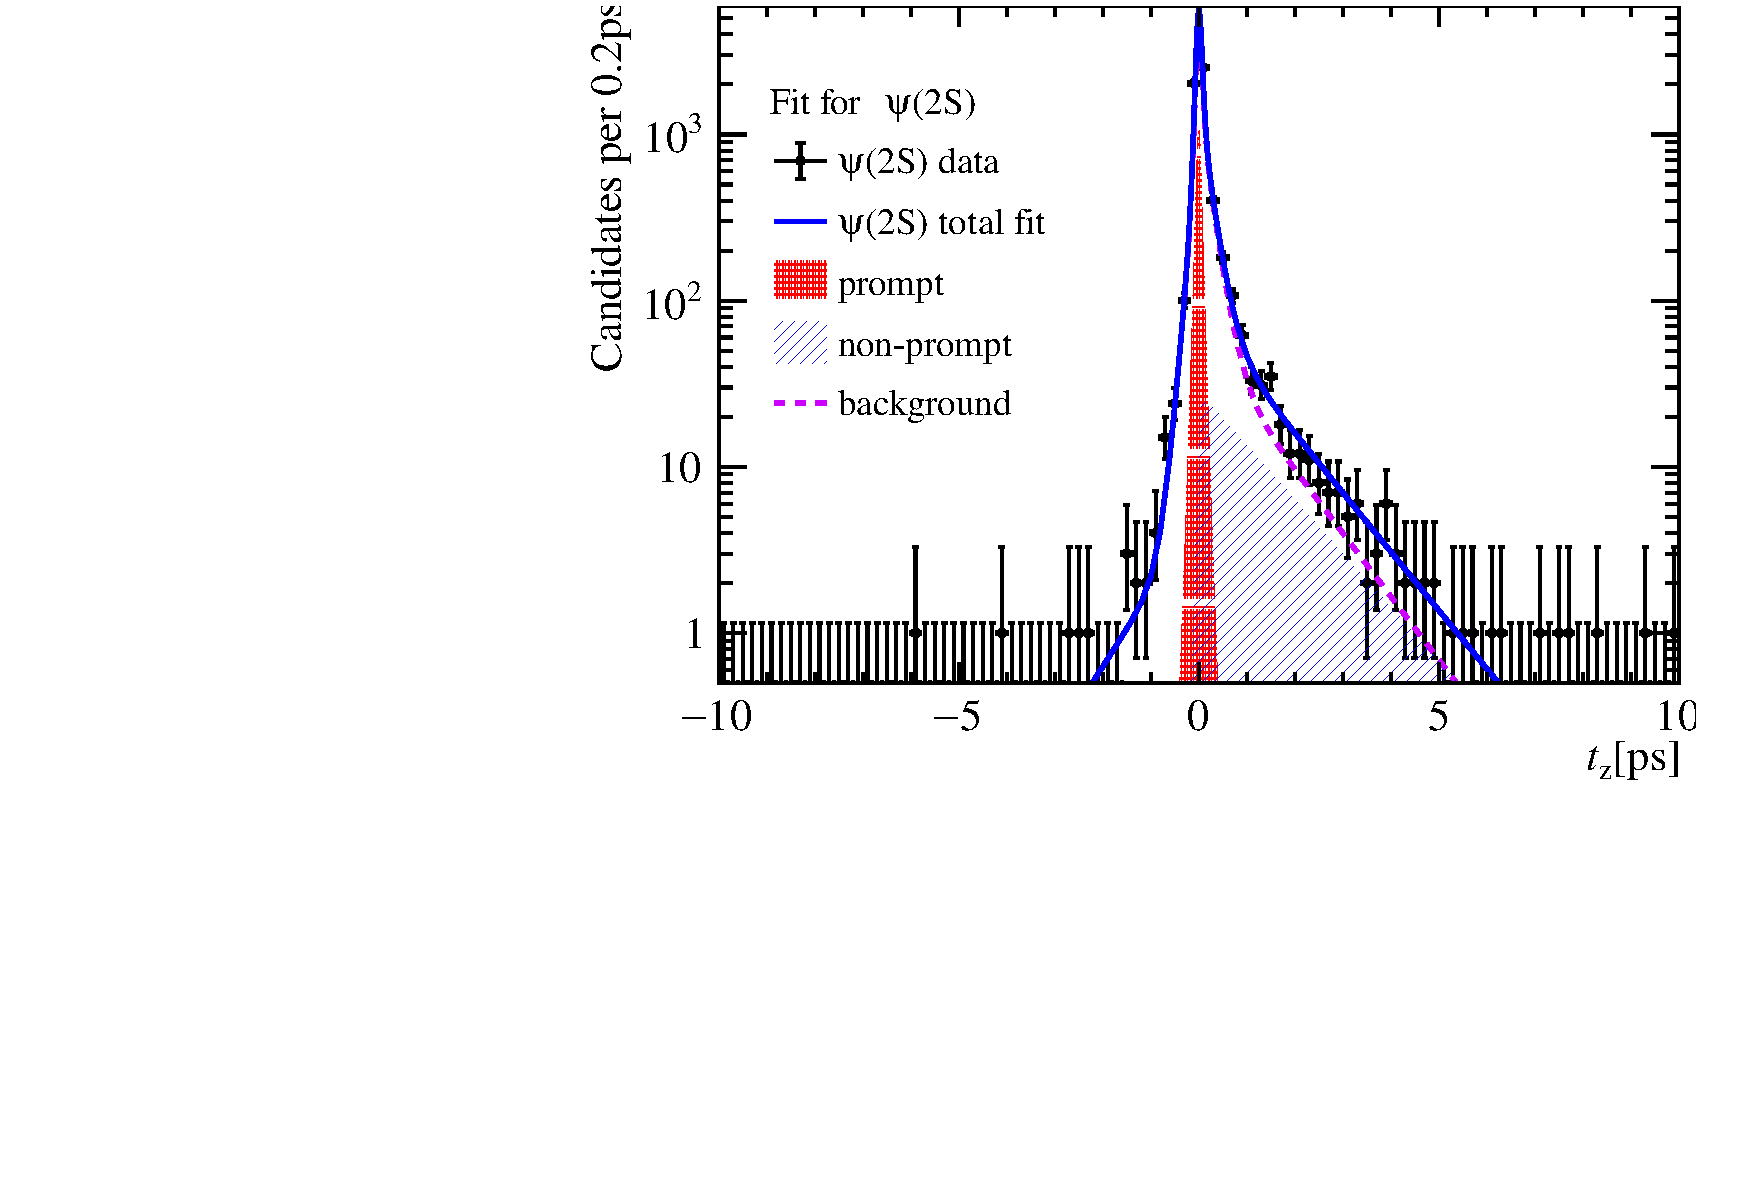
\includegraphics[width=0.49\linewidth]{pdf/pPb/Workdir/TwoDimFit/ProjTz/Psi2S_n2y1pt1.pdf}
    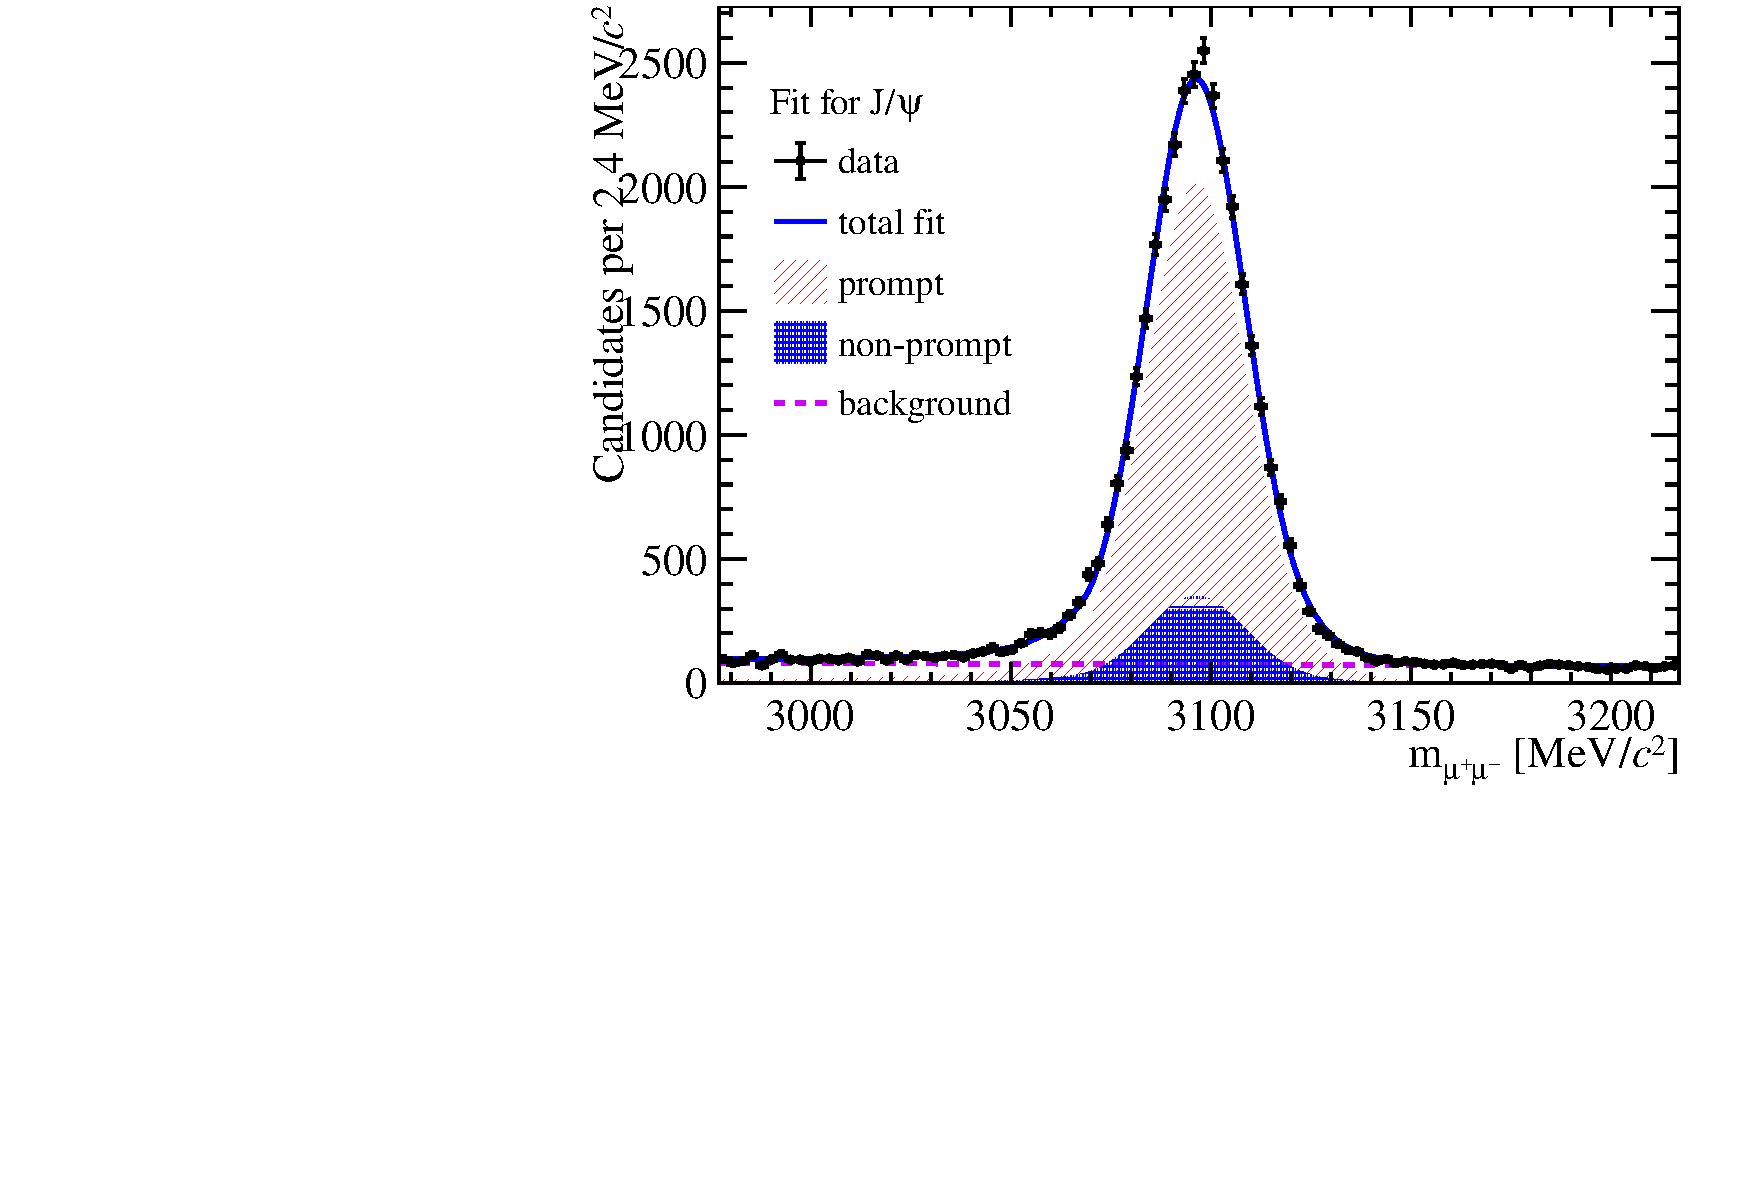
\includegraphics[width=0.49\linewidth]{pdf/pPb/Workdir/TwoDimFit/ProjMass/Jpsi_n2y1pt1.pdf}
    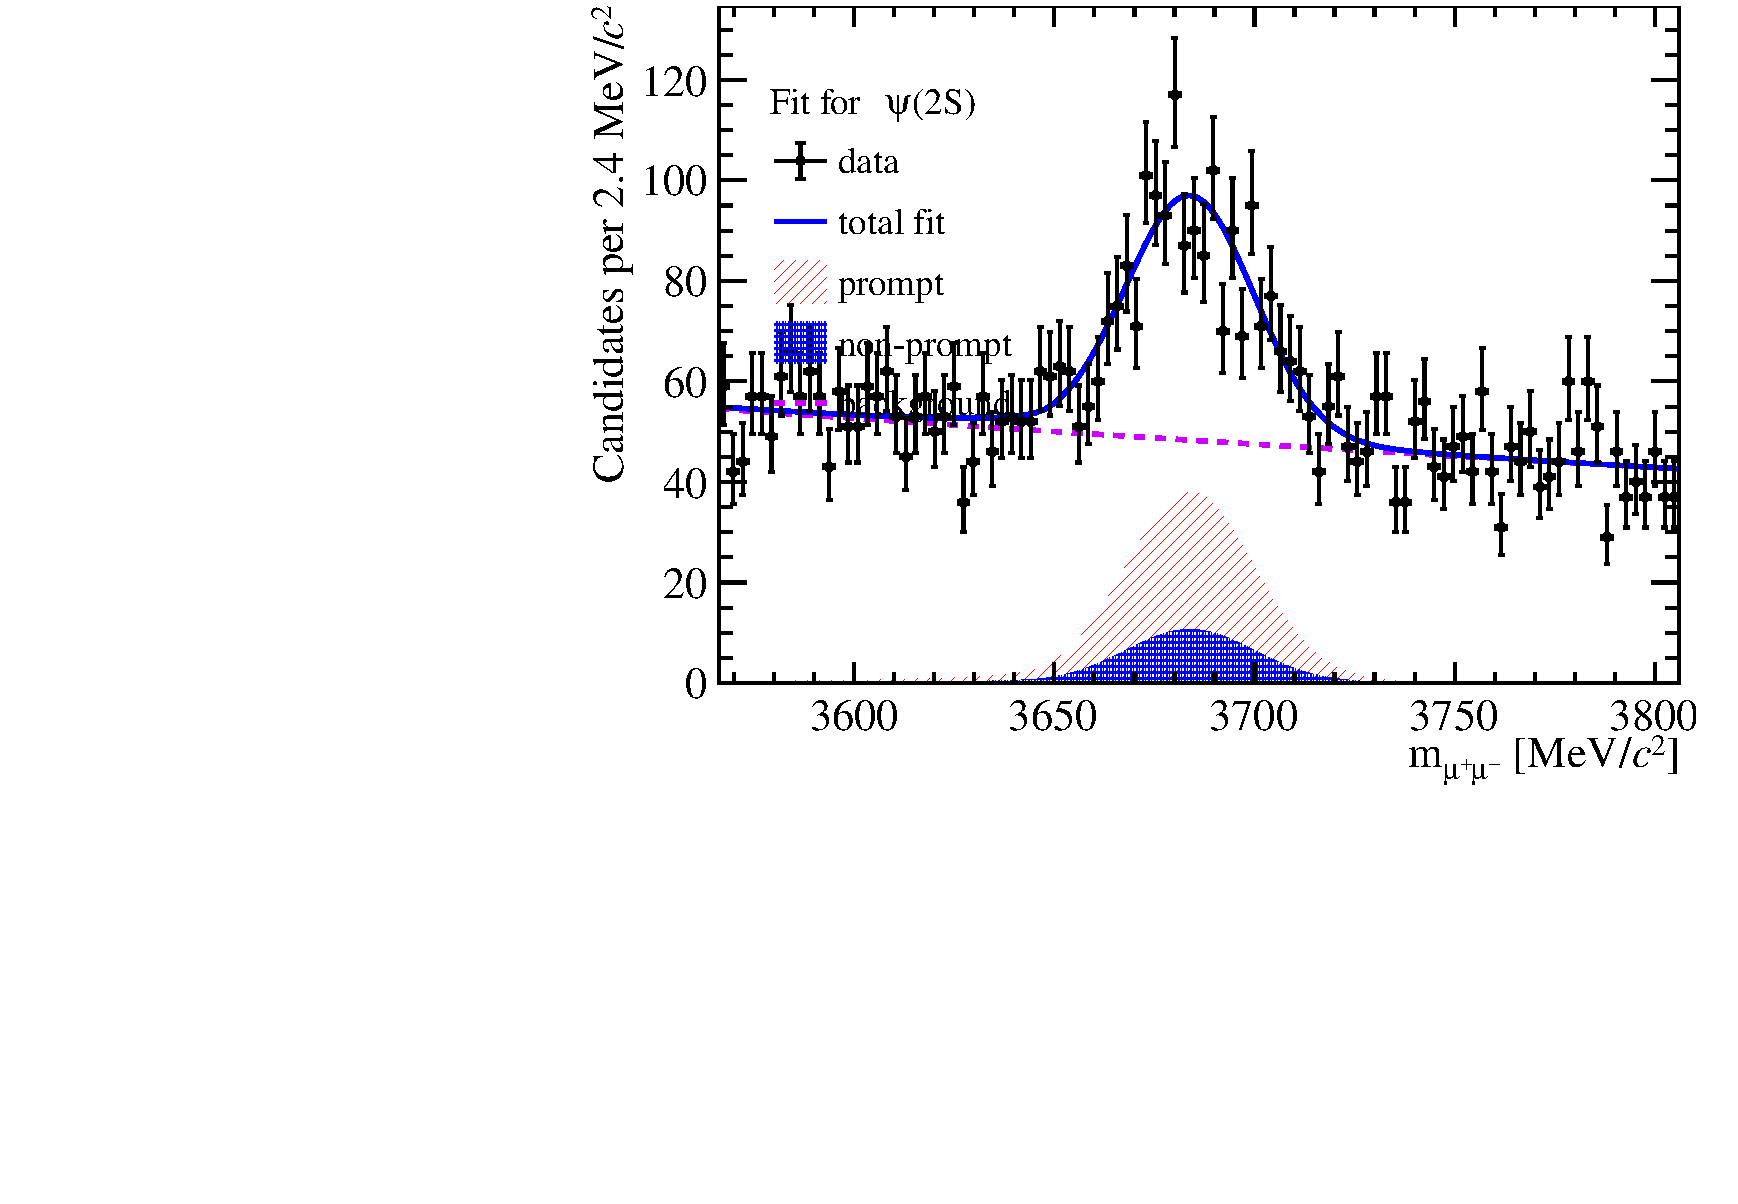
\includegraphics[width=0.49\linewidth]{pdf/pPb/Workdir/TwoDimFit/ProjMass/Psi2S_n2y1pt1.pdf}
  \end{center}
  \caption{
    Two-dimensional fit projected on mass and $t_z$ spectrum for 45$\leq$$N^{\rm PV}_{\rm tracks}$$<$70, $1.5<y^*<4.5$, and $0<\pt<14\gevcc$ for $p$Pb configuration. The left is that of $\jpsi$ and the right is of $\psitwos$.
    }
  \label{fig:2Dtz}
\end{figure}


